\section{Fundamentos}
\label{recifragem:fundamentos}
A recifragem por \emph{proxy} [\cite{blaze1998divertible}] é uma alternativa ao esquema criptográfico assimétrico tradicional [\cite{1363std}] que permite a delegação de direitos de acesso a messagens cifradas de maneira eficiente e mais segura. Em um cenário tradicional caso o usuário \emph{u}1 queira que somente os usuários \emph{u}2 e \emph{u}3 tenham acesso a suas mensagens cifradas ele primeiro cifra suas mensagens com sua chave privada (\emph{sk}1), em seguida cifra novamente com as chaves de \emph{u}2 e \emph{u}3 separadamente, de forma que ao distribuir essa mensagem cada um com suas respectivas chaves privadas e a chave pública de \emph{u}1 poderá decifrar a mensagem.

Em cenários onde se tem uma certa volatilidade quanto aos usuários e que a mensagem a ser transmitida não altera com tanta frequência, ou seja, existe mais mudanças de usuários que do conteúdo da mensagem. A abordagem tradicional de criptografia assimétrica se mostra uma abordagem pouco eficiente, visto que para cada vez que um usuário diferente necessitar consumir o conteúdo será necessário recifrar a mensagem a ser transmitida usando sua respectiva chave pública (\emph{pk}n) de forma que somente ele consiga reproduzi-la. Uma outra abordagem possível é através da entrega da chave privada de \emph{u}1 à \emph{u}n [\cite{ma2009group}]. Porém essa abodargem apresenta grande desvantagem visto que \emph{u}n terá acesso a chave privada de \emph{u}1 e por consequência terá acesso a todas as suas mensagens e por isso deve ser uma entidade confiável de \emph{u}1[\cite{libert2011unidirectional}].

A recifragem por \emph{proxy} explora as adptações do modelo tradicional introduzindo um novo elemento, o \emph{proxy}, que será responsável por intermediar a validação de chaves entre o usuário \emph{u}1 e seus consumidores. Simplificando é como se o \emph{proxy} agora fosse o responsável por fornecer as chaves de acesso ao conteúdo gerado por \emph{u}1 sem que o mesmo precise fornecer sua chave privada ou mesmo ter que recifrar todo o conteúdo com a chave pública dos usuários que irão consumir o mesmo.

Neste sistema o usuário \emph{u}1 irá cifrar seu conteúdo uma vez e o enviará para o \emph{proxy}. Paralelamente será gerado uma chave de recifragem que também será enviada ao \emph{proxy}. Dentro deste o conteúdo será recifrado utilizando agora a chave de recifragem de \emph{u}1 para \emph{u}n. Essa chave de recifragem permitirá ao usuário \emph{u}n decifrar o conteúdo recifrado pelo \emph{proxy} com a sua respectiva chave privada (\emph{pk}n) confome podemos observar na figura:
\begin{figure}[H]
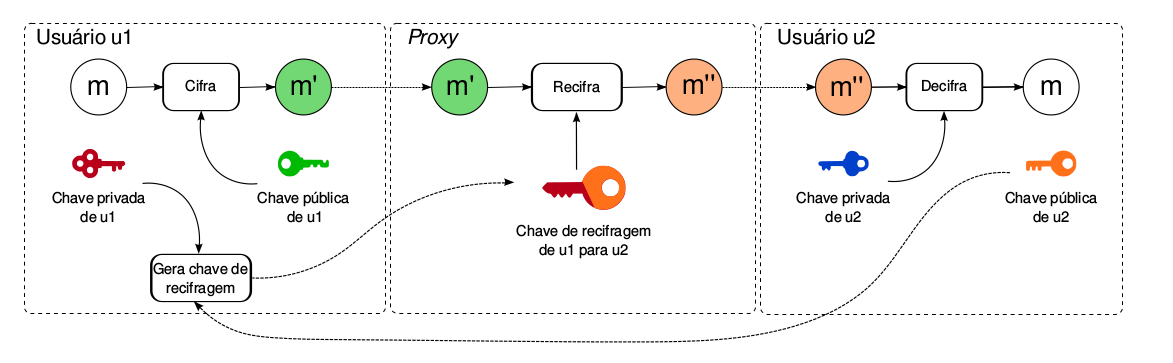
\includegraphics[width=17cm]{Figuras/recifragemPorProxy.png}
\caption{Recifragem por \emph{proxy} (\cite{mannes2016controle})} 
\label{figura:contextualizacao} 
\end{figure}

Há algumas premissas de operações padrão do esquemas de recifragem por \emph{proxy}. A implementação dos mesmos vai depender do tipo de recifragem[\cite{ateniese2006improved}, \cite{chow2010efficient}]:

\textit{Configuração:} recebe como entrada um parâmetro de segurança \emph{k} e tem como saída uma tupla de parâmetros globais. 

\textit{Geração de chaves:} gera os pares de chaves pública, \emph{pk}, e privada, \emph{sk}.

\textit{Cifragem:} recebe pk(u1) e uma mensagem m, gera uma mensagem {m}pk(u1).

\textit{Geração de chave de recifragem:} tem como entrada a chave privada sk(u1) e a chave pública pk(u2) e como saída uma chave de recifragem rku1!u2.

\textit{Recifragem:} recebe a chave de recifragem rku1!u2 e o texto cifrado {m}pk(u1) , tem como saída {m}pk(u2) .

\textit{Decifragem} utilizando sk(u2) e {m}pk(u2) , gera como saída a mensagem m.

Afim de que o método seja considerado seguro foram incorporado diversas propriedades que respeitam 3 asserções básicas: (1) o \emph{proxy} não pode ser capaz de acessar o conteúdo da mensagem que recifra; (2) o usuário \emph{u}2 não pode obter o conteúdo da mensagem sem a interveção da função de recifragem; (3) O \emph{proxy} não pode, em hipótese nenhuma, obter as chaves privadas em posse das chave de recifragem e da mensagem cifrada[\cite{matsuo2007proxy},\cite{zhu2010new}].

Um resumo das possíveis caractéristicas de uma recifragem por \emph{proxy} está definido na tabela.

% ######## init table ########
%% ######## init table ########

\begin{table}[!htp]
\begin{tabular}{|c|c|c|}
\hline
Propriedades & Valores & Descrição \\ \hline
\multirow{Direção da delegação} & Unidirecional  & a  delegação $u1 \rightarrow u2$ não implica na delegação de $u2 \rightarrow u1$ \\ \cline{2-2}\cline{3-3} 
& Bidirecional  & a delegação u1 → u2 implica na delegação de u2 → u1 \\ \hline

\multirow{Número de saltos de recifragrem} & Único Salto \centering & somente mensagens originais podem ser recifradas \\ \cline{2-2}\cline{3-3} 
& Multiplos Saltos \centering & uma mensagem recifrada de u1 → u2 pode ser novamente recifrada de u2 → u3 \\ \hline

\multirow{Transitividade da chave de recifragem} & Transitivo & descrição transitivo \\ \cline{2-2}\cline{3-3} 
& Intransitivo \centering & o proxy não pode, a partir de rk u1→u2 e rk u2→u3 ,produzir rk u1→u3 \\ \hline

\multirow{Necessidade de iteração com o usuário} & Iterativo \centering & as chaves de recifragem são geradas por u1 com a necessidade de interações com u2 \\ \cline{2-2}\cline{3-3} 
& Não iterativo \centering & as chaves de recifragem são geradas por u1 sem a necessidade de interações com u2 \\ \hline

\multirow{Robustez contra conluio} & Robusto \centering & o usuário u2 e o proxy em conluio não conseguem recuperar a chave privada de u1 \\ \cline{2-2}\cline{3-3} 
& Não robusto \centering & o usuário u2 e o proxy em conluio conseguem recuperar a chave privada de u1 \\ \hline
\end{tabular}
\caption{Propriedades dos esquemas de recifragem por \textit{proxy}}
\label{table}
\end{table}

A recifragem por \emph{proxy} gerou então diversas abordagens com combinações mistas de propriedades. Dentro dessas abordagens está \emph{Efficient Unidirectional Proxy Re-Encryption} (EU-PRE) [\cite{chow2010efficient}] que contempla as seguintes propriedades: (1) \textit{Unirediconal}, (2) \textit{Único salto}, (3) \textit{Intrasitivo}, (4) \textit{Interativo} e (5) \textit{Robusto contra coluio}.

Outros duas abordagens também se encaixam nessas mesmas propriedades: são elas o esquema de \emph{proxy} invisível[\cite{jia2010cca}] e o esquema de \emph{proxy} anônimo [\cite{shao2012anonymous}]. Dessas três abordagens o EU-PRE se mostra mais simples e eficente, pois não implementa as funções de anonimato das mensagens cifradas e nem as funções de invisibilidade do \emph{proxy}.

Além disso, o trabalho de \cite{mannes2016controle} apresenta uma nova abordagem quanto ao EU-PRE. Retirando do sistema a necessidade de ter um agente de \emph{proxy}  sem impactar na segurança do processo.

Esse processo é feito através da otimização das equações matemáticas onde o processo de cifragem ainda ficará com o provedor de conteúdo e os de decifragem e recifragem ficarão a cargo do usuário. Eliminando assim um terceiro elemento do sistema, o que torna-o muito mais parecido com os que temos hoje.